% LearningToOptimize ecosystem: the type hierarchy of L2OCore.
%
% Methods (by family, plus wrappers that add behaviour to any method), problem
% classes (traits detected from the JuMP model) and evaluators (interchangeable
% batched backends). Abstract types are plain navy names; concrete types are
% chips; dashed chips are planned. Concrete types live in L2OCore
% (SupervisedMSE, BoundedOutput, ProjectionRepair, the classes and evaluators),
% LearningToOptimize (PenaltyMethod), L2OSobolev (SobolevRegularized) and the
% method packages (DC3 and FSNet in L2ODC3, DualLagrangianLearning in L2ODLL,
% ALMMethod in L2OALM). Content follows docs/src/design.md.
%
% Build: make -C docs/src/assets/diagrams/src
%   pdflatex -jobname=learningtooptimize--types types.tex          -> wide layout
%   pdflatex -jobname=learningtooptimize--types-compact types.tex  -> narrow layout
\documentclass[tikz,border=4pt]{standalone}
% Shared style of the LearningToOptimize diagrams: the palette, lane frames, cards,
% chips and glyphs of the paper-style TikZ figures (the same visual system as the
% PortfolioOpt.jl and DecisionRules.jl figures). Each figure \input's this file.
\usepackage{amsmath,amssymb,bm}
\usepackage[T1]{fontenc}
\usepackage[scaled=0.92]{helvet}
\renewcommand{\familydefault}{\sfdefault}
\usetikzlibrary{arrows.meta,shapes.geometric,shapes.symbols,calc,positioning,decorations.pathreplacing}

\definecolor{dTeal}{HTML}{1A9AA0}
\definecolor{dTealLine}{HTML}{3FB3B8}
\definecolor{dNavy}{HTML}{3F4C8C}
\definecolor{dInk}{HTML}{1E2235}
\definecolor{dRed}{HTML}{E4573D}
\definecolor{dCoral}{HTML}{E2765A}
\definecolor{dOrange}{HTML}{F4A93B}
\definecolor{dPeach}{HTML}{FBD9AC}
\definecolor{dPanel}{HTML}{EEF0F2}
\definecolor{dGray}{HTML}{8A90A0}
\definecolor{dNode}{HTML}{14A3A8}
\definecolor{dShadow}{HTML}{D5DAE3}

% \ifcompact is true when the job name ends in "-compact" (narrow layout).
\newif\ifcompact
\ifnum\pdfmatch{-compact$}{\jobname}=1 \compacttrue\fi

\tikzset{
  >={Stealth[length=5pt,width=4pt]},
  every node/.style={text=dInk},
  title/.style={anchor=west,font=\small,inner sep=0pt},
  head/.style={font=\small\bfseries,text=dNavy},
  note/.style={font=\itshape\footnotesize,text=dNavy},
  dnote/.style={font=\itshape\footnotesize,text=dCoral},
  code/.style={font=\ttfamily\footnotesize,text=dNavy},
  store/.style={cylinder,shape border rotate=90,aspect=0.28,fill=dPeach,draw=dOrange,
                line width=0.7pt,minimum width=0.95cm,minimum height=1.2cm,font=\normalsize},
  dia/.style={diamond,fill=dOrange,draw=none,minimum size=0.9cm,inner sep=0pt,aspect=1,
              font=\normalsize},
  lnode/.style={circle,fill=dRed,draw=none,minimum size=0.66cm,inner sep=1pt,
                text=white,font=\normalsize},
  card/.style={rectangle,rounded corners=4pt,fill=white,draw=dShadow,line width=0.6pt},
  sheet/.style={rectangle,rounded corners=3pt,fill=dPanel,draw=dShadow,line width=0.6pt},
  chip/.style={rectangle,rounded corners=3pt,fill=dPanel,draw=none,font=\small,
               inner xsep=4pt,inner ysep=3pt},
  ochip/.style={chip,fill=white,draw=dGray,dashed,line width=0.6pt},
  pchip/.style={chip,fill=white,draw=dGray!70,dashed,line width=0.5pt,text=dGray},
  fwd/.style={->,dTealLine,line width=0.8pt},
  tgt/.style={->,dOrange,line width=0.9pt},
  dual/.style={->,dCoral,dashed,line width=0.9pt},
  dep/.style={->,dTealLine,line width=0.8pt},
  pdep/.style={->,dGray,dashed,line width=0.7pt},
  nn/.style={circle,minimum size=0.26cm,inner sep=0pt,draw=dInk!70,line width=0.35pt},
}

% Lane frame in the paper style: two shadow copies behind a teal rounded frame.
\newcommand{\lane}[4]{% #1 x0, #2 y0, #3 x1, #4 y1
  \foreach \o/\c in {0.16/dShadow!60,0.08/dShadow}
    \draw[\c,fill=white,rounded corners=5pt,line width=0.6pt]
      (#1+\o,#2-\o) rectangle (#3+\o,#4-\o);
  \draw[dTealLine,fill=white,rounded corners=5pt,line width=0.9pt] (#1,#2) rectangle (#3,#4);}

% Plain card frame (no shadow copies), for problems and losses.
\newcommand{\cardbox}[4]{\draw[dShadow,fill=white,rounded corners=4pt,line width=0.6pt] (#1,#2) rectangle (#3,#4);}

% Network glyph on one sheet. #1 = centre, #2 = name prefix, #3 = number of stacked
% sheets behind (0, 1 or 2).
\newcommand{\net}[3]{%
  \begin{scope}[shift={(#1)}]
    \ifnum#3>1 \node[sheet,minimum width=1.9cm,minimum height=1.8cm] at (0.30,0.22) {};\fi
    \ifnum#3>0 \node[sheet,minimum width=1.9cm,minimum height=1.8cm] at (0.15,0.11) {};\fi
    \node[sheet,minimum width=1.9cm,minimum height=1.8cm,fill=white] (#2sheet) at (0,0) {};
    \foreach \y [count=\i] in {0.36,0,-0.36} \node[nn,fill=dGray!45] (#2in\i) at (-0.64,\y) {};
    \foreach \y [count=\i] in {0.58,0.29,0,-0.29,-0.58} \node[nn,fill=dNode] (#2ha\i) at (-0.21,\y) {};
    \foreach \y [count=\i] in {0.44,0.15,-0.15,-0.44} \node[nn,fill=dNode] (#2hb\i) at (0.21,\y) {};
    \node[nn,fill=dOrange] (#2out) at (0.64,0) {};
    \foreach \a in {1,...,3} \foreach \b in {1,...,5} \draw[dGray!60,line width=0.2pt] (#2in\a) -- (#2ha\b);
    \foreach \a in {1,...,5} \foreach \b in {1,...,4} \draw[dGray!60,line width=0.2pt] (#2ha\a) -- (#2hb\b);
    \foreach \a in {1,...,4} \draw[dGray!60,line width=0.2pt] (#2hb\a) -- (#2out);
  \end{scope}}

% Jacobian mask glyph: an n x d grid with a few entries selected. #1 = centre.
\newcommand{\maskgrid}[1]{%
  \begin{scope}[shift={(#1)}]
    \foreach \i in {0,...,4} \foreach \j in {0,...,3}
      \draw[dShadow,fill=white,line width=0.4pt] (\j*0.2-0.4,-\i*0.2+0.5) rectangle ++(0.2,-0.2);
    \foreach \i/\j in {0/1,1/3,2/0,3/2,4/1}
      \draw[dOrange,fill=dOrange,line width=0.4pt] (\j*0.2-0.4,-\i*0.2+0.5) rectangle ++(0.2,-0.2);
  \end{scope}}

% Code names inside italic notes stay upright.
\newcommand{\cmd}[1]{{\upshape\ttfamily #1}}

% Software-architecture helpers: package cards, type chips and chip rows.
\tikzset{
  pkg/.style={rectangle,rounded corners=4pt,fill=white,draw=dShadow,line width=0.6pt,
              align=center,inner xsep=5pt,inner ysep=4pt,font=\footnotesize},
  pkgcore/.style={pkg,draw=dTealLine,line width=0.9pt},
  pkgplan/.style={pkg,draw=dGray,dashed,text=dGray},
  tchip/.style={chip,font=\ttfamily\footnotesize,inner xsep=3pt,inner ysep=2.5pt},
  tplan/.style={tchip,fill=white,draw=dGray,dashed,line width=0.5pt,text=dGray},
  absname/.style={anchor=west,font=\ttfamily\footnotesize,text=dNavy,inner sep=1pt},
}
% \chiprow{x}{y}{style}{A,B,C}: chips left to right from (x,y), anchored west.
\newcommand{\chiprow}[4]{%
  \coordinate (cr@next) at (#1,#2);
  \foreach \t in {#4} {%
    \node[#3,anchor=west] (cr@last) at (cr@next) {\t};
    \coordinate (cr@next) at ($(cr@last.east)+(0.12,0)$);}}


% a branch of a tree: horizontal tick from the trunk at x=#1 to the item at y=#2
\newcommand{\tick}[2]{\draw[dGray,line width=0.5pt] (#1,#2) -- (#1+0.3,#2);}

\begin{document}
\ifcompact
% ============================ narrow (phone) layout ============================
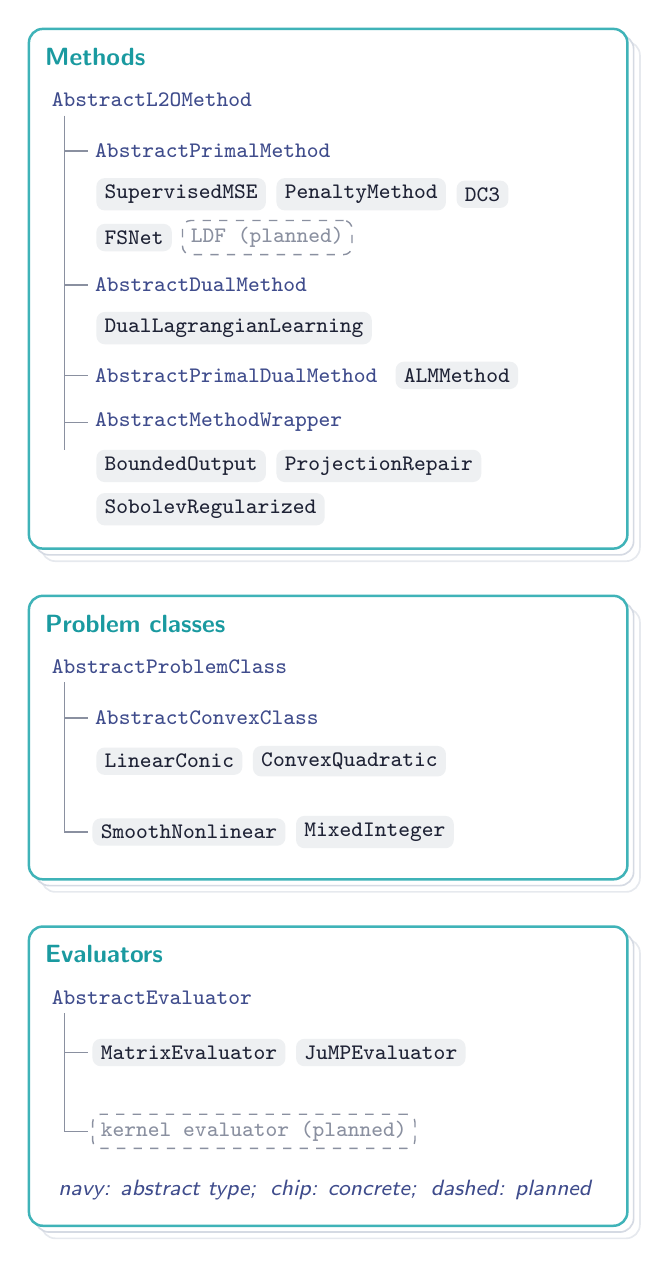
\begin{tikzpicture}
  % ---- methods ----
  \lane{0}{8.6}{7.6}{15.2}
  \node[title] at (0.2,14.85) {\textcolor{dTeal}{\bfseries Methods}};
  \node[absname] at (0.25,14.3) {AbstractL2OMethod};
  \draw[dGray,line width=0.5pt] (0.45,14.1) -- (0.45,9.85);
  \tick{0.45}{13.65}\node[absname] at (0.8,13.65) {AbstractPrimalMethod};
  \chiprow{0.85}{13.1}{tchip}{SupervisedMSE,PenaltyMethod,DC3}
  \chiprow{0.85}{12.55}{tchip}{FSNet}
  \node[tplan,anchor=west] at ($(cr@last.east)+(0.12,0)$) {LDF (planned)};
  \tick{0.45}{11.95}\node[absname] at (0.8,11.95) {AbstractDualMethod};
  \chiprow{0.85}{11.4}{tchip}{DualLagrangianLearning}
  \tick{0.45}{10.8}\node[absname] at (0.8,10.8) {AbstractPrimalDualMethod};
  \chiprow{4.65}{10.8}{tchip}{ALMMethod}
  \tick{0.45}{10.2}\node[absname] at (0.8,10.2) {AbstractMethodWrapper};
  \chiprow{0.85}{9.65}{tchip}{BoundedOutput,ProjectionRepair}
  \chiprow{0.85}{9.1}{tchip}{SobolevRegularized}
  % ---- problem classes ----
  \lane{0}{4.4}{7.6}{8.0}
  \node[title] at (0.2,7.65) {\textcolor{dTeal}{\bfseries Problem classes}};
  \node[absname] at (0.25,7.1) {AbstractProblemClass};
  \draw[dGray,line width=0.5pt] (0.45,6.9) -- (0.45,5.0);
  \tick{0.45}{6.45}\node[absname] at (0.8,6.45) {AbstractConvexClass};
  \chiprow{0.85}{5.9}{tchip}{LinearConic,ConvexQuadratic}
  \tick{0.45}{5.0}\chiprow{0.8}{5.0}{tchip}{SmoothNonlinear,MixedInteger}
  % ---- evaluators ----
  \lane{0}{0}{7.6}{3.8}
  \node[title] at (0.2,3.45) {\textcolor{dTeal}{\bfseries Evaluators}};
  \node[absname] at (0.25,2.9) {AbstractEvaluator};
  \draw[dGray,line width=0.5pt] (0.45,2.7) -- (0.45,1.2);
  \tick{0.45}{2.2}\chiprow{0.8}{2.2}{tchip}{MatrixEvaluator,JuMPEvaluator}
  \tick{0.45}{1.2}\chiprow{0.8}{1.2}{tplan}{kernel evaluator (planned)}
  \node[note,anchor=west] at (0.25,0.45) {navy: abstract type;\; chip: concrete;\; dashed: planned};
\end{tikzpicture}
\else
% =============================== wide layout ===================================
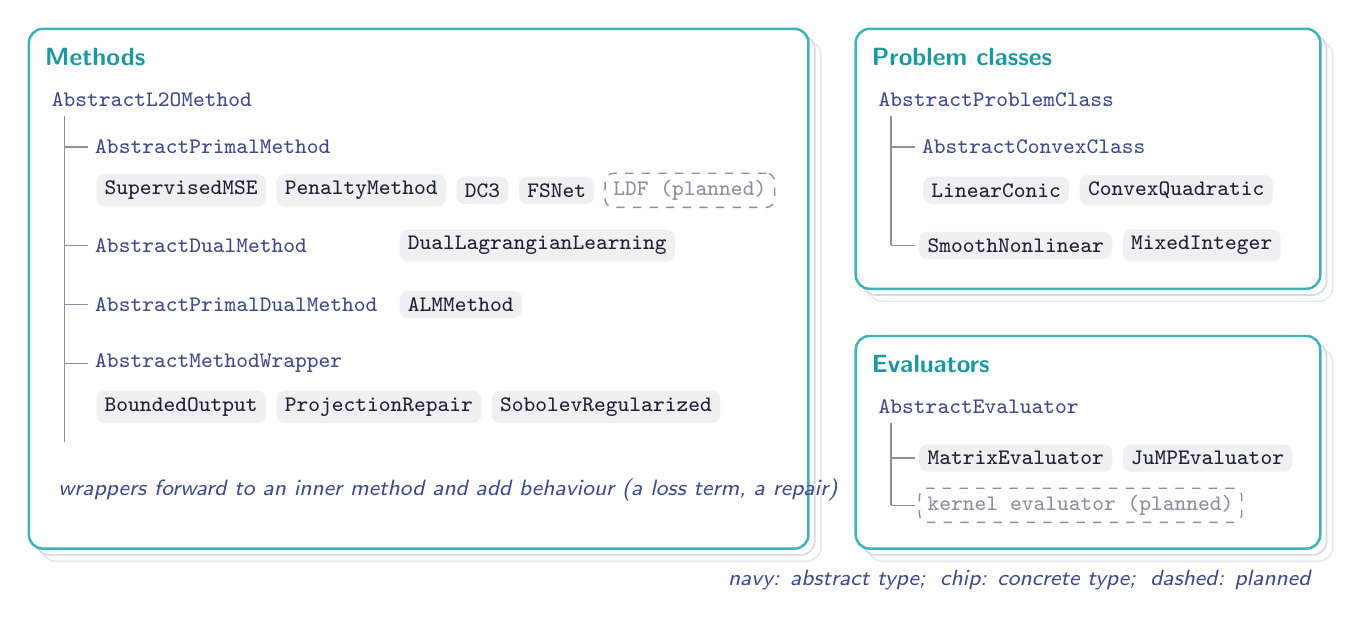
\begin{tikzpicture}
  % ---- methods ----
  \lane{0}{0}{9.9}{6.6}
  \node[title] at (0.2,6.25) {\textcolor{dTeal}{\bfseries Methods}};
  \node[absname] at (0.25,5.7) {AbstractL2OMethod};
  \draw[dGray,line width=0.5pt] (0.45,5.5) -- (0.45,1.35);
  \tick{0.45}{5.1}\node[absname] at (0.8,5.1) {AbstractPrimalMethod};
  \chiprow{0.85}{4.55}{tchip}{SupervisedMSE,PenaltyMethod,DC3,FSNet}
  \node[tplan,anchor=west] at ($(cr@last.east)+(0.12,0)$) {LDF (planned)};
  \tick{0.45}{3.85}\node[absname] at (0.8,3.85) {AbstractDualMethod};
  \chiprow{4.7}{3.85}{tchip}{DualLagrangianLearning}
  \tick{0.45}{3.1}\node[absname] at (0.8,3.1) {AbstractPrimalDualMethod};
  \chiprow{4.7}{3.1}{tchip}{ALMMethod}
  \tick{0.45}{2.35}\node[absname] at (0.8,2.35) {AbstractMethodWrapper};
  \chiprow{0.85}{1.8}{tchip}{BoundedOutput,ProjectionRepair,SobolevRegularized}
  \node[note,anchor=west] at (0.25,0.75) {wrappers forward to an inner method and add behaviour (a loss term, a repair)};
  % ---- problem classes ----
  \lane{10.5}{3.3}{16.4}{6.6}
  \node[title] at (10.7,6.25) {\textcolor{dTeal}{\bfseries Problem classes}};
  \node[absname] at (10.75,5.7) {AbstractProblemClass};
  \draw[dGray,line width=0.5pt] (10.95,5.5) -- (10.95,3.85);
  \tick{10.95}{5.1}\node[absname] at (11.3,5.1) {AbstractConvexClass};
  \chiprow{11.35}{4.55}{tchip}{LinearConic,ConvexQuadratic}
  \tick{10.95}{3.85}\chiprow{11.3}{3.85}{tchip}{SmoothNonlinear,MixedInteger}
  % ---- evaluators ----
  \lane{10.5}{0}{16.4}{2.7}
  \node[title] at (10.7,2.35) {\textcolor{dTeal}{\bfseries Evaluators}};
  \node[absname] at (10.75,1.8) {AbstractEvaluator};
  \draw[dGray,line width=0.5pt] (10.95,1.6) -- (10.95,0.55);
  \tick{10.95}{1.15}\chiprow{11.3}{1.15}{tchip}{MatrixEvaluator,JuMPEvaluator}
  \tick{10.95}{0.55}\chiprow{11.3}{0.55}{tplan}{kernel evaluator (planned)}
  \node[note,anchor=east] at (16.4,-0.4) {navy: abstract type;\; chip: concrete type;\; dashed: planned};
\end{tikzpicture}
\fi
\end{document}
